\documentclass[sigconf,review=false,anonymous=false]{acmart}
\settopmatter{printacmref=false}
\setcopyright{none}
\acmConference[CS 544 Project]{CS 544 Machine Learning in Production}{Fall 2026}{University of Illinois Chicago}
\acmYear{2026}\acmDOI{}\acmISBN{}
\renewcommand\footnotetextcopyrightpermission[1]{}
\pagestyle{plain}
\usepackage{booktabs}
\usepackage{multirow}
\usepackage{xspace}
\usepackage{graphicx}
\graphicspath{{../report/figures/}}
\setlength{\emergencystretch}{1.5em}

\begin{document}

\title{When Should an LLM Issue Triager Stay Silent? Calibration, Drift, Rewording and Evidence in Issue Triage}

\author{Sina Gogani-Khiabani}
\affiliation{\institution{University of Illinois Chicago}\city{Chicago}\state{IL}\country{USA}}
\email{sgoga3@uic.edu}
\author{Verya Monjezi}
\affiliation{\institution{University of Illinois Chicago}\city{Chicago}\state{IL}\country{USA}}
\author{Third Author}
\affiliation{\institution{University of Illinois Chicago}\city{Chicago}\state{IL}\country{USA}}

\begin{abstract}
Issue-labeling services now apply LLM labels to open-source issues automatically. We evaluate one
as a deployed, selective service: Qwen2.5-7B, zero-shot and with retrieved examples, against
classical classifiers, on the NLBSE'24 benchmark and on 1{,}430 issues the same five repositories
received in 2025--26, after the model's training cutoff. The classical TF-IDF classifier is the most
accurate on the benchmark (76.2\%) but falls to 67.5\% on 2025--26 issues and 60.3\% on a new
repository; the LLM is stable (70.9\%, 75.3\%, 68.0\%). Raw LLM probabilities are badly overconfident.
A confidence threshold tuned for 10\% error among auto-labeled issues overshoots in every condition
(14.9\% in distribution, 20.5\% on a new repository); a risk-controlled threshold keeps the target in
distribution and a year later but auto-labels only 7\% of issues, and no threshold carries over to a
new repository. A one-sentence newcomer apology flips 16.2\% of the few-shot LLM's labels, mostly
toward question, and non-native English costs the zero-shot LLM up to 10 points; calibrated deferral
keeps almost all such flips from being auto-applied. The LLM's evidence quotes are genuine (93\%
verbatim) but deleting them moves its decision little more than deleting random text. Input novelty
detects a new repository within 11 requests, while the model's own confidence rarely notices. A
record/replay regression suite catches injected bugs in calibration, retrieval and preprocessing.
\end{abstract}

\keywords{issue triage, large language models, selective prediction, calibration, robustness, explanations, ML in production}

\maketitle

\section{Introduction}

Open-source projects receive more issues than maintainers can read, and automatic labeling is one of
the most requested forms of help. GitHub now ships an LLM-based labeler as an
Action~\cite{github2025labeler}, and research has moved from fine-tuned classifiers to
LLMs~\cite{colavito2025issue,aracena2025issue}. Benchmarks report how often a labeler is right on a
fixed snapshot~\cite{nlbse24}. A deployed labeler faces different questions. Which labels should it
apply on its own, and which should it leave for a person? Does its promised error rate hold a year
later, or on a repository it has never seen? Does it treat a report differently because the reporter
writes in non-native English or apologizes for being new? And when it explains a decision, is the
explanation what actually drove it?

We study these questions with a triage service built around Qwen2.5-7B, running locally, on the
NLBSE'24 benchmark (3{,}000 issues from five large repositories, 2016--2023) and on 1{,}430 issues the
same repositories received in 2025--2026, after the model's training cutoff. We compare the LLM,
zero-shot and with retrieved examples, against classical classifiers trained on the repositories'
history, and ask:
\begin{description}
\item[RQ1] How do classical and LLM triagers compare in distribution, a year later, and on a new
repository?
\item[RQ2] Can calibrated deferral keep the error among auto-applied labels at a target (10\%), and
does that promise survive drift?
\item[RQ3] Do meaning-preserving changes in how an issue is written (no stack trace, no template, a
newcomer apology, non-native English) change the label?
\item[RQ4] Are the evidence quotes the LLM gives faithful to its decision?
\item[RQ5] Which logged signal notices that the stream of issues has changed?
\end{description}

The answers are mixed in useful ways. A TF-IDF classifier trained on the history is the most accurate
in distribution (76.2\%) but drops to 67.5\% on 2025--26 issues and 60.3\% on a new repository; the
LLM is less accurate in distribution (70.9\%) but stable (75.3\% and 68.0\%). Raw LLM label
probabilities are badly overconfident (fitted temperatures of 8--10). A confidence threshold tuned to
10\% error on calibration data overshoots in every condition (14.9\% in distribution, 20.5\% on a new
repository); a risk-controlled threshold keeps the promise in distribution and a year later but
auto-labels only 7\% of issues. A one-sentence newcomer apology flips 16.2\% of the few-shot LLM's
labels, mostly toward \emph{question}, yet calibrated deferral keeps almost all flips from being
auto-applied. The LLM's evidence quotes are real quotes, but deleting them moves its decision little
more than deleting random text. A simple novelty signal, distance to the closest labeled history
issue, detects a new repository within 11 requests; the model's own confidence rarely notices.

\paragraph{Contributions.} (1) An evaluation of LLM issue triage as a deployed, selective service,
including a post-cutoff 2025--26 set from the benchmark's own repositories; (2) evidence that common
calibration recipes over-promise and that rigorous risk control is affordable only with far more
calibration data; (3) behavioral tests showing a newcomer-apology sensitivity that in-context examples
amplify; (4) a faithfulness test of LLM triage explanations; and (5) monitoring and record/replay
regression tests for the service, all on one laptop.

\section{Related Work}\label{sec:related}

\paragraph{Issue classification.} Ticket Tagger predicts GitHub issue types from text with
fastText~\cite{kallis2021tickettagger}. The NLBSE tool competitions turned the task into a shared
benchmark; the 2024 edition provides 3{,}000 balanced issues from five repositories and a SetFit
baseline~\cite{nlbse24}. Colavito et al.\ benchmark 22 decoder LLMs against fine-tuned
encoders and find zero-shot LLMs less consistent across datasets~\cite{colavito2025issue}; Aracena
et al.\ compare GPT-4o and DeepSeek-R1 on the same data~\cite{aracena2025issue}. GitHub now ships an
LLM-based issue labeler as an Action~\cite{github2025labeler}. These works report accuracy on a fixed
benchmark; we ask how a deployed labeler should decide when \emph{not} to label, and what happens
after the benchmark period.

\paragraph{Calibration and selective prediction.} Modern networks are overconfident, and temperature
scaling is a simple fix~\cite{guo2017calibration}. Selective classification abstains below a
confidence threshold chosen for a target risk~\cite{geifman2017selective}; split conformal
prediction gives distribution-free coverage under exchangeability~\cite{angelopoulos2021conformal}.
We test whether these guarantees survive the shifts a triage service meets in production.

\paragraph{Behavioral testing, fairness and explanations.} CheckList tests NLP models with
meaning-preserving perturbations~\cite{ribeiro2020checklist}. LLMs answer users with lower English
proficiency less accurately~\cite{poole2024llm}, which motivates testing whether a triager treats
non-native reporters differently. ERASER measures whether rationales are faithful by deleting
them~\cite{deyoung2020eraser}; we apply the same idea to the evidence quotes an LLM triager gives.

\paragraph{ML in production.} Monitoring, calibration under drift, and regression tests are part of
production readiness~\cite{breck2017mltestscore,kastner2025mlip}.

\section{Study Design}\label{sec:design}

\subsection{The triage service}
The service receives a new GitHub issue and either applies one label (\emph{bug}, \emph{feature},
\emph{question}) or leaves the issue for a maintainer. Bodies are preprocessed as a deployed service
would: HTML comments left by issue templates are removed and the body is cut to 1{,}500 characters.
We compare four classifiers. Two are classical: TF-IDF features with logistic regression, and
\texttt{bge-small-en-v1.5}~\cite{xiao2023cpack} embeddings with logistic regression. Two use
Qwen2.5-7B-Instruct~\cite{qwen2025qwen25} (4-bit, MLX~\cite{mlx2023}, one laptop): \emph{zero-shot}
with label definitions, and \emph{few-shot}, which adds the six most similar labeled issues from the
same repository, retrieved by embedding similarity. For the LLMs we read the next-token distribution
after the prompt and take the probability mass on each label word, renormalized over the three
labels; this costs one prefill pass and needs no verbalized confidence.

\subsection{Data and conditions}
\emph{NLBSE'24}~\cite{nlbse24} supplies 3{,}000 issues (react, tensorflow, vscode, bitcoin,
opencv; 2016--2023; 100 per repository and label in each half). We split its training half into a
labeled history of 1{,}005 issues (training data for the classical models and retrieval pool for the
few-shot LLM) and a calibration split of 495, and use its full test half (1{,}500 issues). We
evaluate three conditions:
\begin{description}
\item[In-distribution:] the NLBSE'24 test set.
\item[Fresh 2025--26:] issues created between January 2025 and October 2026 in the same five
repositories, collected with the GitHub API and mapped to the three labels through each repository's
own label names (1{,}430 single-type issues; a balanced sample of up to 40 per repository and label,
514 issues). History and calibration stay in 2016--2023, as for a service deployed and not
retrained; the period also lies after the model's training cutoff, which removes benchmark leakage.
\item[New repository:] 750 test issues triaged as if their repository had just been onboarded: the
few-shot model retrieves examples only from the other four repositories and the classical models are
trained without the target repository.
\end{description}

\subsection{Selective automation}
Each classifier's scores are temperature-scaled~\cite{guo2017calibration} on the calibration split.
We compare five policies: \emph{auto-all}; a \emph{naive threshold} on calibrated confidence, the
lowest one whose auto-labeled calibration issues have at most 10\% errors~\cite{geifman2017selective};
a \emph{risk-controlled threshold} chosen by Learn-then-Test~\cite{angelopoulos2021ltt}, which tests
thresholds from the most confident down and accepts each while a 95\% Clopper--Pearson upper bound on
its calibration error stays at or below 10\%;
\emph{conformal}, which auto-labels only when the split-conformal prediction set at $\alpha{=}0.1$ has
one label~\cite{angelopoulos2021conformal}; and \emph{agreement}, which auto-labels only when the
few-shot LLM and the embedding classifier agree. Thresholds and conformal quantiles are set once on
the calibration split and applied unchanged in every condition.

\subsection{Rewording tests}
From the test set we draw 210 probe issues (14 per repository and label) and create five
meaning-preserving variants each: \emph{no code} (fenced blocks and stack-trace lines removed),
\emph{no template} (template headings and checklists removed), \emph{newcomer} (a sentence saying
the reporter is new and apologizing for a possibly silly question), \emph{non-native} (the prose
rewritten as by a non-native English speaker; code blocks are masked during rewriting and restored),
and \emph{non-native + no code}. The non-native rewrite is produced by Llama-3.2-3B~\cite{grattafiori2024llama3},
a different model family from the classifier under test, and kept only if every code block is
restored, the length stays within 0.5--1.8$\times$, and at least 80\% of technical tokens survive. A
label flip between an issue and its variant is a robustness failure, because the issue type is
unchanged by construction.

\subsection{Explanations}
For the probe issues the few-shot model is also asked for its label and two exact quotes from the
issue as evidence. We check whether the quotes occur verbatim and run a deletion
test~\cite{deyoung2020eraser}: the issue is re-scored, with the same retrieved examples, after
deleting the quoted text and, as a control, after deleting random spans of the same total length
(two seeds).

\subsection{Statistics}
Intervals are percentile bootstraps over issues (2{,}000 resamples). Monitoring follows the protocol
of Section~\ref{sec:monitor}.

\section{Results}\label{sec:results}

\begin{table}[t]
\caption{Accuracy (\%) by condition and cross-repository F1. Tokens: prompt tokens per issue.}\label{tab:acc}
\small
\begin{tabular}{lrrrr}
\toprule
Approach & NLBSE'24 & 2025--26 & New repo & Tokens \\
\midrule
TF-IDF + LR & 75.5 & 66.3 & 60.4 & -- \\
Embedding + LR & 69.3 & 68.5 & 57.5 & -- \\
LLM zero-shot & 68.5 & 71.2 & 68.4 & 0.4k \\
LLM few-shot & 70.9 & 75.3 & 68.0 & 1.1k \\
\midrule
\multicolumn{5}{l}{\emph{Cross-repository F1 (NLBSE ranking metric)}} \\
TF-IDF + LR & 0.754 & 0.583 & 0.592 & \\
Embedding + LR & 0.691 & 0.630 & 0.561 & \\
LLM zero-shot & 0.663 & 0.650 & 0.661 & \\
LLM few-shot & 0.694 & 0.682 & 0.657 & \\
\bottomrule
\end{tabular}

\end{table}

\subsection{RQ1: Accuracy in and out of distribution}
Table~\ref{tab:acc}. In distribution, TF-IDF with logistic regression, trained on only 1{,}005
labeled issues, is the most accurate approach (76.2\%, 95\% CI [74.0, 78.3]); the few-shot LLM reaches
70.9\% [68.6, 73.3] and zero-shot 68.5\%. Out of distribution the order reverses. On 2025--26 issues
TF-IDF drops to 67.5\% and its cross-repository F1 from 0.760 to 0.584, while the few-shot LLM rises to
75.3\%. On a new repository TF-IDF and the embedding classifier fall to 60.3\% and 58.8\%; the LLMs
lose at most 3 points (68.0\%, 68.4\%). The classical models learn repository- and period-specific
vocabulary; the LLM relies on general knowledge of what bugs, features and questions look like.

The 2025--26 issues also serve as a leakage control: they postdate the model's training data, and the
LLM is \emph{more} accurate on them than on the 2016--2023 benchmark, so we see no sign that benchmark
contamination inflates LLM results here. The fresh data show a different kind of drift instead:
label usage. React, for example, labeled 200 bugs but only 9 feature requests and 5 questions in
2025--26, since it now routes questions elsewhere, so a labeler tuned to the benchmark's balanced
classes faces a very different prior.

\begin{figure*}[t]
\centering
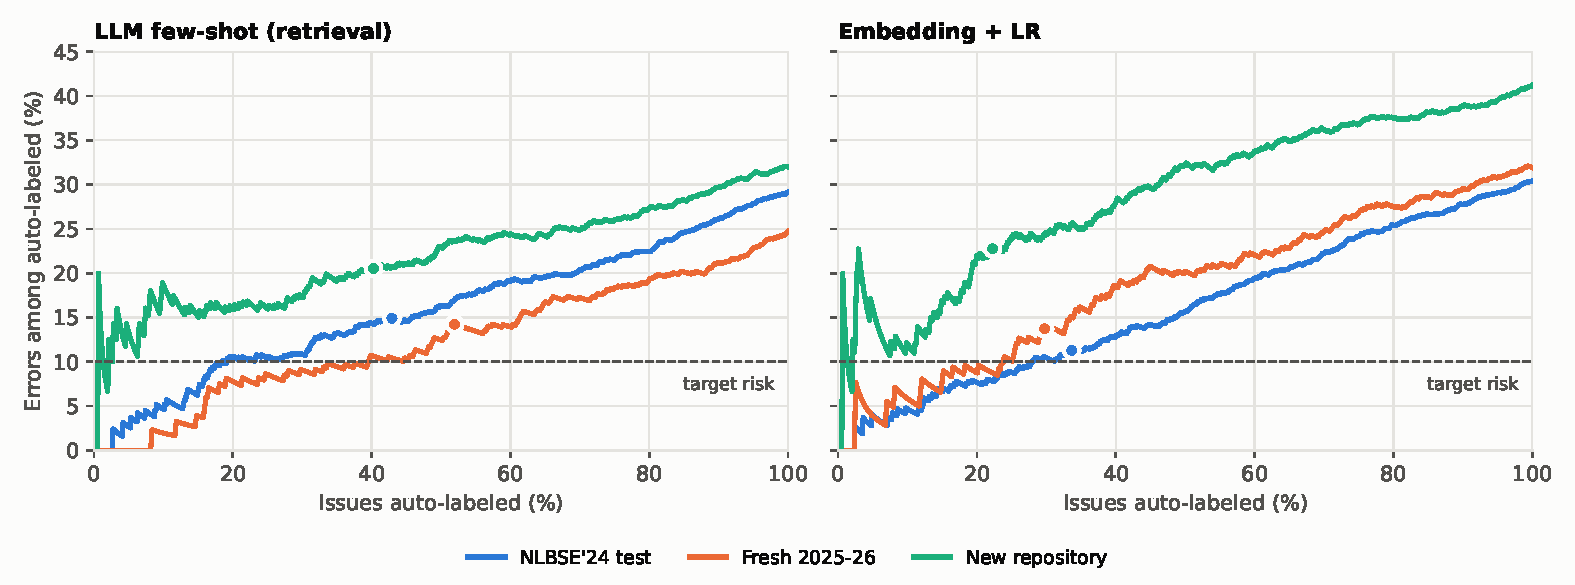
\includegraphics[width=0.92\textwidth]{risk_coverage.pdf}
\caption{Risk--coverage curves: error among the most confident issues as more are auto-labeled.
Dots: the naive threshold calibrated for 10\% error. The dashed line is the target.}\label{fig:rc}
\end{figure*}

\begin{table*}[t]
\caption{Selective automation: coverage / risk (\%), i.e., share auto-labeled / errors among them.
Target risk: 10\%. All thresholds are set on the calibration split.}\label{tab:sel}
\small
\begin{tabular}{llrrr}
\toprule
Approach & Policy & NLBSE'24 & 2025--26 & New repo \\
\midrule
TF-IDF + LR & auto-all & 100.0 / 23.8 & 100.0 / 32.5 & 100.0 / 39.7 \\
 & naive threshold & 54.9 / 12.5 & 48.8 / 19.1 & 33.5 / 26.3 \\
 & risk-controlled & 15.6 / 4.3 & 12.5 / 9.4 & 1.5 / 18.2 \\
 & conformal & 61.9 / 14.5 & 60.7 / 23.7 & 46.5 / 28.9 \\
\midrule
Embedding + LR & auto-all & 100.0 / 30.4 & 100.0 / 31.9 & 100.0 / 41.2 \\
 & naive threshold & 33.7 / 11.3 & 29.8 / 13.7 & 22.3 / 22.8 \\
 & risk-controlled & 13.5 / 5.9 & 11.5 / 5.1 & 8.0 / 11.7 \\
 & conformal & 47.7 / 15.7 & 44.7 / 18.3 & 38.5 / 28.7 \\
\midrule
LLM zero-shot & auto-all & 100.0 / 31.5 & 100.0 / 28.8 & 100.0 / 31.6 \\
 & naive threshold & 13.1 / 12.2 & 24.9 / 7.8 & 10.9 / 14.6 \\
 & risk-controlled & 0.0 / -- & 0.0 / -- & 0.0 / -- \\
 & conformal & 29.5 / 17.8 & 39.3 / 11.4 & 27.1 / 17.2 \\
\midrule
LLM few-shot & auto-all & 100.0 / 29.1 & 100.0 / 24.7 & 100.0 / 32.0 \\
 & naive threshold & 42.9 / 14.9 & 51.9 / 14.2 & 40.3 / 20.5 \\
 & risk-controlled & 6.9 / 3.9 & 8.0 / 0.0 & 1.2 / 11.1 \\
 & conformal & 52.8 / 17.9 & 59.5 / 16.3 & 50.5 / 22.7 \\
\midrule
LLM few-shot + Emb. & agreement & 67.0 / 17.8 & 71.4 / 17.7 & 63.6 / 26.4 \\
\bottomrule
\end{tabular}

\end{table*}

\subsection{RQ2: Does calibrated deferral keep its promise?}
Raw LLM label probabilities are almost always 0 or 1; temperature scaling on the calibration split
needs $T{=}7.6$ (few-shot) and $T{=}10.1$ (zero-shot) and lowers expected calibration error from
0.23--0.30 to 0.05--0.08. The classical models are underconfident ($T{\approx}0.6$).

Table~\ref{tab:sel} and Figure~\ref{fig:rc} show what happens when the scores are used to decide
which issues to label automatically. The \emph{naive threshold} --- the lowest threshold at which the
auto-labeled calibration issues contain at most 10\% errors --- overshoots the target in every
condition, even in distribution (TF-IDF 12.5\%, few-shot LLM 14.9\%), and badly under shift (TF-IDF
26.3\%, LLM 20.5\% on a new repository). Choosing a threshold on 495 calibration issues is optimistic
by construction: the lowest feasible threshold sits where calibration noise happens to look good.
The \emph{risk-controlled} threshold keeps the promise in distribution (3.9--5.9\% risk) and on
2025--26 issues (0--9.4\%), but it pays with coverage: the few-shot LLM auto-labels only 6.9\% of
issues, the zero-shot LLM none, and TF-IDF 15.6\%. On a new repository it fails for every classifier
that auto-labels anything (11.1--18.2\%), because the guarantee assumes calibration and deployment
data are exchangeable. In hindsight, the test data would have allowed auto-labeling 19.1\% of issues
at 10\% error with the few-shot LLM and 45.5\% with TF-IDF; on a new repository no threshold reaches
10\% for any trained classifier. With 495 calibration issues, the naive rule overshoots that point and
the rigorous rule stops far short of it. Conformal prediction sets cover the true label in
87.5--89.3\% of in-distribution cases (target 90\%); on a new repository the classical classifiers
fall to 80.0--83.5\%, while the LLMs stay at 86--89\% in every condition. An
agreement gate between the LLM and the embedding classifier labels about two thirds of issues at
17.7--26.4\% risk, far from the target.

\begin{table}[t]
\caption{Label flips (\%) under meaning-preserving rewording of 210 probe issues (\emph{n}:
applicable variants), and accuracy change.}\label{tab:rob}
\small
\setlength{\tabcolsep}{3.5pt}
\resizebox{\columnwidth}{!}{\begin{tabular}{lrrrrr}
\toprule
Approach & No code & No templ. & Newcomer & Non-native & NN + no code \\
\midrule
\emph{n} & 77 & 112 & 210 & 159 & 159 \\
TF-IDF + LR & 13.0 & 13.4 & 7.1 & 13.2 & 17.0 \\
Embedding + LR & 5.2 & 12.5 & 6.2 & 8.2 & 9.4 \\
LLM zero-shot & 3.9 & 0.0 & 5.7 & 6.9 & 10.1 \\
LLM few-shot & 6.5 & 3.6 & 16.2 & 7.5 & 9.4 \\
\midrule
\multicolumn{6}{l}{\emph{Accuracy change, original $\to$ variant (points)}} \\
TF-IDF + LR & -1.3 & +4.5 & -2.9 & -0.6 & -3.8 \\
Embedding + LR & -5.2 & +0.0 & +2.9 & -2.5 & -3.8 \\
LLM zero-shot & -3.9 & +0.0 & -2.4 & -6.9 & -10.1 \\
LLM few-shot & +0.0 & -1.8 & -3.3 & -4.4 & -5.0 \\
\bottomrule
\end{tabular}
}
\end{table}

\subsection{RQ3: Does the way an issue is written change its label?}
Table~\ref{tab:rob} and Figure~\ref{fig:flips}. TF-IDF is the most fragile: removing code, removing
template scaffolding or rewriting in non-native English each flips 13--17\% of its labels. The LLMs
are more robust to style and structure, with one striking exception: a single sentence in which the
reporter says they are new and apologizes for a possibly silly question flips 16.2\% of the few-shot
LLM's labels, 14.8\% toward \emph{question}, against 5.7\% for zero-shot. The effect does not come
through retrieval: 85\% of the retrieved examples are unchanged and the share of question examples
stays at 0.33. In-context examples make the model more sensitive to the cue itself. Non-native English
costs the zero-shot LLM 6.9 points of accuracy, and 10.1 points when the stack trace is also missing,
which matters for reporters who rely on logs because their English is limited.

Deferral absorbs almost all of this: with the naive threshold, the share of variants where both the
original and the rewritten issue would be auto-labeled with different labels is 0--1.3\% for every
classifier. Flips happen among issues the service was already unsure about.

\begin{figure}[t]
\centering
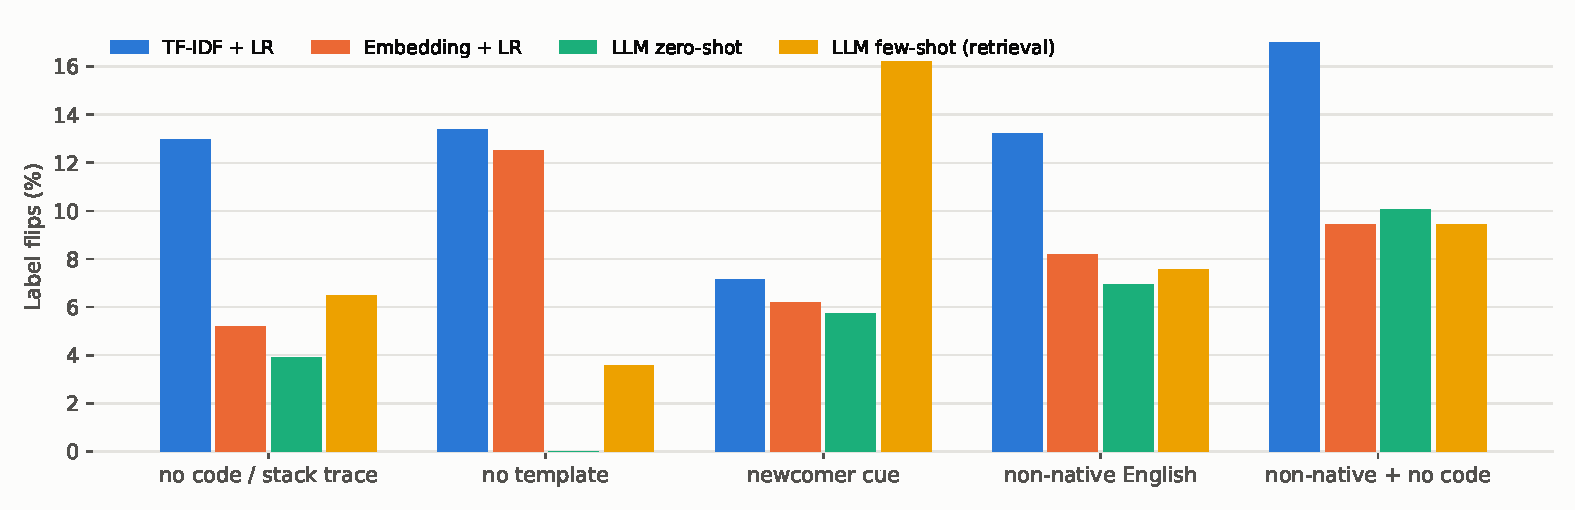
\includegraphics[width=\columnwidth]{flips.pdf}
\caption{Label flips under rewording.}\label{fig:flips}
\end{figure}

\subsection{RQ4: Are the explanations faithful?}
Asked for a label and two exact quotes as evidence, the few-shot LLM quoted the issue in 178 of 210
cases; 93.1\% of its 331 quotes occur verbatim, and the explained label matches the scored label in
92.9\% of issues. Faithfulness is weaker. On 164 issues with locatable quotes (on average 130 of 921
body characters), deleting the quoted evidence lowered the calibrated probability of the predicted
label by 0.025, against 0.014 for deleting random text of the same length (Wilcoxon $p{=}0.115$); it
changed the label in 6.1\% of issues against 3.0\% for random deletion, and lowered confidence more than
random deletion in only 55.5\% of issues. The quotes are plausible and real, but the decision is spread
across the issue and the retrieved examples; they should not be presented as \emph{the} reason.

\subsection{RQ5: Which signal notices a changed stream?}\label{sec:monitor}
We simulate 300 streams per shift: 400 in-distribution requests, then 200 from 2025--26, from a
repository without history, or in non-native English. A signal alarms when its rate over the last 50
requests exceeds the in-distribution mean plus three standard deviations. Table~\ref{tab:mon} and
Figure~\ref{fig:mon}: \emph{novelty}, one minus the cosine similarity to the closest labeled history
issue the service may retrieve from, detects a new repository a median of 11 requests after the shift
and 2025--26 traffic after 38 (98\% of runs), with no false alarms. The model's own signals --- share
handed to a human, low confidence, disagreement with the embedding classifier --- detect these shifts
in under a third of runs, and the predicted-label distribution in at most half. No signal reliably
notices the non-native stream. Model-confidence monitoring alone would miss drift that input
monitoring catches immediately.

\begin{table}[t]
\caption{Detection delay after a shift: median requests to the first alarm (share of 300 runs
detected); --: detected in fewer than half.}\label{tab:mon}
\small
\setlength{\tabcolsep}{4pt}
\resizebox{\columnwidth}{!}{\begin{tabular}{lrrrrr}
\toprule
Shift & Handoff & Low conf. & Disagree & Novelty & Label shift \\
\midrule
2025--26 issues & -- & -- & -- & 38 (98\%) & -- \\
New repository & -- & -- & -- & 11 (100\%) & -- \\
Non-native & -- & -- & -- & -- & -- \\
\bottomrule
\end{tabular}
}
\end{table}

\begin{figure*}[t]
\centering
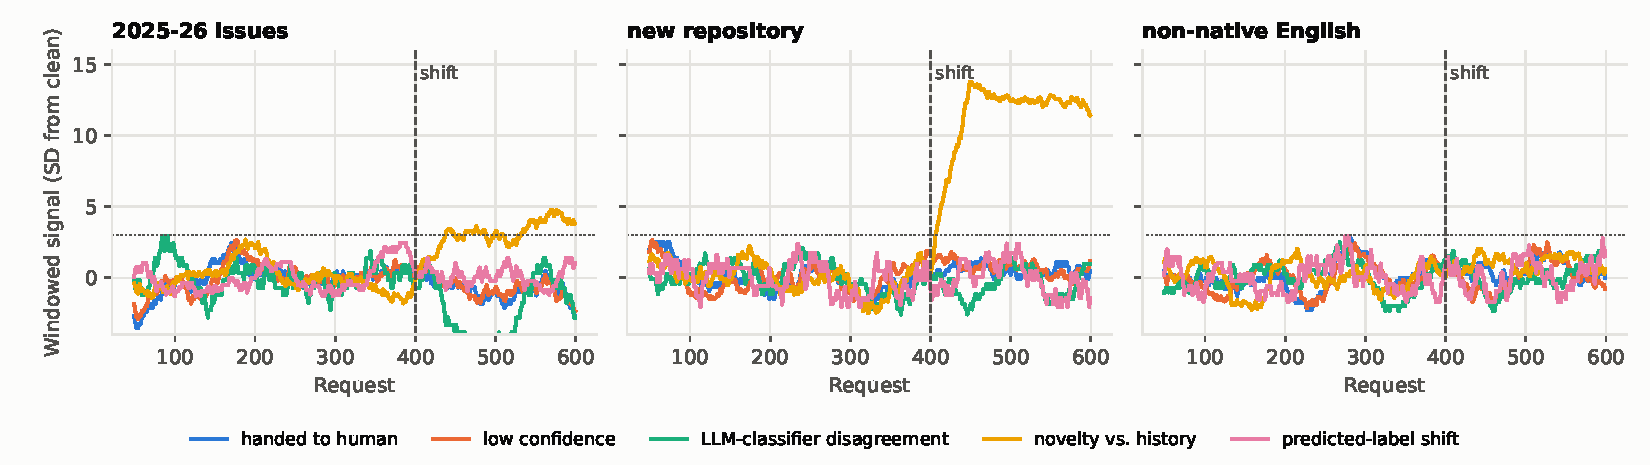
\includegraphics[width=0.92\textwidth]{monitoring.pdf}
\caption{Windowed signals in one simulated stream per shift, standardized against the clean segment;
the dotted line is the alarm level.}\label{fig:mon}
\end{figure*}

\subsection{Regression tests}
A 40-case suite (issues auto-labeled correctly, wrong predictions that must be handed off, and
rewrites that must keep their label) replays the full pipeline from recorded model scores in about 6
seconds. Injecting plausible bugs and replaying live: removing temperature scaling fails 14 cases
(every must-hand-off case is then auto-labeled), retrieving examples from other repositories fails
10, cutting the issue body to 300 characters fails 6, dropping retrieval fails 5, and removing the
label definitions from the prompt fails only 1, a gap in the suite.

\section{Lessons for Practitioners}

\paragraph{Benchmark accuracy is the wrong selection criterion.} The most accurate classifier on the
benchmark was the least accurate a year later and on a new repository. Evaluate a labeler on issues
from after its training and calibration data, and on a held-out repository, before choosing it.

\paragraph{A calibrated threshold is not an error guarantee.} Tuning the threshold to the target on a
few hundred calibration issues over-promised in every condition. A risk-controlling procedure needs
its threshold candidates fixed before certification, and with 330 certification issues it certified
a 10\% target only for the classical classifier and at low coverage. Choose the target from a
frontier like Table~\ref{tab:frontier}, or budget for far more labeled calibration issues. A
certificate holds only for data exchangeable with the calibration set: recalibrate, on that
repository's own labeled issues, when a repository is onboarded.

\paragraph{Calibration across repositories fixes sets, not thresholds.} Leave-one-repository-out
calibration brought conformal coverage back to about 88--92\% on a new repository, but naive
thresholds still overshot. Prediction sets, which keep a human in the loop for ambiguous issues,
transfer better than a single auto-label threshold.

\paragraph{Deferral protects labels, not reporters.} Flips under rewording concentrate where the
service is unsure, so almost none are auto-applied. But a reporter who calls their post ``a silly
question'' is auto-labeled half as often and waits for a human instead. Measure workload and wait
time by reporter group, not only flips, and keep reporter self-descriptions out of the classifier's
input where possible.

\paragraph{Show evidence as context, not as cause.} The LLM's quotes are genuine, but we could not
show that they matter more than other text; a triage UI should present them as relevant passages,
not as the reason for the label.

\paragraph{Monitor inputs, not only the model.} A nearest-neighbor novelty score over the labeled
history caught a new repository within 13 requests at under 1\% false alarms; the model's confidence
did not, and disagreement between models alarmed falsely in 5--7\% of clean windows.

\section{Threats to Validity}\label{sec:threats}

\paragraph{Construct.} Labels are the repositories' own type labels, which mix issue content with
project policy (React routes questions elsewhere). The 2025--26 set maps each repository's label names
to the three types; issues with several type labels are excluded. Rewrites are synthetic. The
non-native rewrite was validated automatically (code blocks restored, length and technical tokens
preserved; 161 of 210 valid) and occasionally alters template fields; a human validation of
meaning preservation on a sample (\texttt{report/audit/rewrite\_audit.csv}) is pending. Removing code
is treated as reduced input, not as a meaning-preserving change. The cue sentences are one wording
each; other phrasings of the same status may behave differently.

\paragraph{Internal.} The calibration issues come from the benchmark's training half and the test set
from its test half, as in the competition. Temperature, threshold candidates and naive thresholds are
fitted on one third of the calibration issues and certified on the other two thirds; nothing is tuned
on test data. All classifiers see the same 1{,}500 characters of each issue. Probabilities are read
from the first output token; a different prompt or label wording would change them.

\paragraph{External.} One LLM, five large repositories, three labels. Smaller projects, other label
sets, and stronger models (including fine-tuned encoders such as the SetFit competition baseline)
may behave differently. The monitoring results come from simulated streams mixed from our pools,
not from a live deployment. All runs used one laptop.

\paragraph{Conclusion validity.} Rewording tests use 77--210 variants per kind; differences of a few
points between classifiers are within noise, while the ``silly question'' effect on the few-shot LLM
is not (paired bootstrap CI [10.0, 20.0]). New-repository results for risk-controlled thresholds rest
on very few auto-labeled issues (TF-IDF: 3 of 750 at the 10\% target) and support no conclusion
beyond the low coverage. The explanation test is underpowered ($p{=}0.115$).

\section{Conclusion}
Treating issue triage as a deployed, selective service changes what matters. The LLM was less
accurate than a simple classifier on the benchmark but held up a year later and on a new repository.
With an honest protocol, a few hundred calibration issues certify a 10\% error rate for almost no
issues, and no certificate carried over to a new repository. A reporter's description of their own
post, not their newcomer status, moved the LLM toward \emph{question}; deferral kept those flips from
being applied but shifted the work to maintainers. The cheapest monitor, input novelty, was the most
useful. The harness, data collection scripts, recorded model scores and regression suite are
available for replication.


\bibliographystyle{ACM-Reference-Format}
\bibliography{refs}

\end{document}
